\subsection{Camera Calibration}

Why do we calibrate?
We want to be aware of the factors within the camera, that may affect the
displaying of our  image.

\textbf{The focal length}, a measure for how much the used lens
centers/bends the light

\begin{figure}[!htbp]
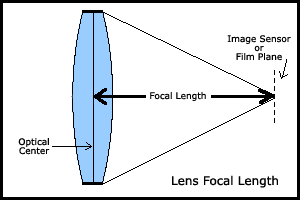
\includegraphics{pics/focal_length.png}
\caption{Focal length}
\label{fig:focal_length}
\end{figure}

\textbf{The image center} (according to the camera), this is not always just
positioned at precisely at half the height, half the width.
\textbf{Scaling factors}. Scaling can occur both horizontally and vertically. 
\textbf{Skew factors}.  Skewing may happen.
\textbf{Lens distortion}.  Cheap lenses may produce pin/cushion effects, and some
cameras may even add additional lenses to correct these issues.

All these factors needs to be taken into consideration when we wish to
calculate projections from the world coordinates to image coordinates. 

We calibrate the camera by using the cv2 implementation and a standard
calibration chessboard pattern. 
